\section{Managing Project Groups} %Jeg skriver kun om admin funktionalitet her -Mikael ~♥
Before any project group can be useful it has to be created first.
Administrators need to have the ability to add, edit, and delete project groups.
The administration tools we provide have to be easy and fast to use, since they potentially have to be used many times.
This section describes how we implemented the administration tools needed to manage project groups.

The features we provide to manage project groups are known as administration tools in Moodle and can be accessed in the site administration menu as seen in \figref{fig:navigation}.

\begin{figure}[htb]
	\centering
		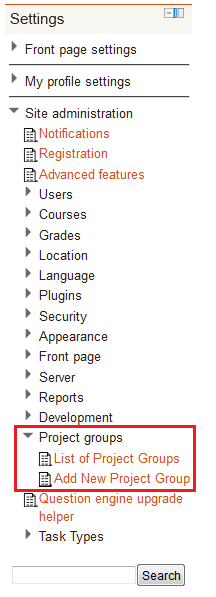
\includegraphics[scale=0.75]{images/admin-navigation.png}
	\morscaption{The settings block, which contains the site administration menu} 
	\label{fig:navigation}
\end{figure}

From here we provide a link to a list of all project groups and a link to a page, from where a new project group can be created.
The page with the list of all project groups has a table with three columns: Short name, Full name, and Actions.
As the name indicates Short name is a short name for a group. 
The Short name also serves as a link to the project group page described in section NEED REF HERERERERER \todo{make a ref to project group page}.
In the Actions column there are links to delete and edit the project group.

The edit page has the same source files as the add page.